\subsubsection{Elastic Sphere}

The analysis of the elastic sphere is more complex, as it necessitates accounting for the indentation between the indenter and the surface and the indentation between the surface and the base. As shown in Figure \ref{fig: Sphere-Sphere-Force_Curve}, the simulations give the characteristic force curve for the indenter and, as before, as the radius of the surface increases, the bounded area decreases. However, from Figure \ref{fig: Sphere-Sphere-Force_Curve-Base}, it can be seen that sampling data at the base of the sphere shows the surface is compressed. However, due to the extremely small indentation, the Hertzian behaviour closely approximates a linear relationship at the base, exhibiting a response consistent with Hooke's Law. 

Moreover, Figure \ref{fig: Sphere-Sphere-Result} shows the indentation of the elastic sphere into the base. Indentation force is distributed between the reaction at the base and the indenter, and part of the perceived indentation depth is due to compression at the base. Therefore, corrected values for the indentation depth is calculated by subtracting the surface compression at its base from the indenter's displacement. Similarly, the corrected forces are the sum of the reaction forces. However, as this research focuses on AFM imaging, the fitted force and indentation data are produced from the indenter data alone, and compression is accounted for using "Double Contact" models\cite{dokukin2013quantitative,glaubitz2014novel}(Appendix \ref{Appendix: Double Contact}).

 For these simulations, the radius of the elastic sphere is varied to test the model's accuracy across varying curvature. Figure \ref{fig: Sphere-Sphere-Contact_Models} shows the difference in the corrected and indenter data. Fitting the contact models to the spherical indenter's data produced tight adherence from the Hertz, Dimitriadis, and Double Contact models. Similarly, for the capped conical indenter, shown in Figure \ref{fig: Capped-Sphere-Contact_Models}, the Hertz, Sneddon, and Double Contact models produced tight fits. In contrast, the Hertz model gave a poor fit for the conical indenter, while the Sneddon and Double Contact models produced tight fits. 

Comparing the fitted Young's modulus variation over surface radius produced various convergent behaviours. The results indicate that the simple Hertzian model underestimates the elastic modulus as the data converged below the expected value for all simple contact models. In contrast, the double contact models converge to the actual value. This highlights the importance of the contribution of compression at the base of the sample. Considering only the indenter data reduces the force experienced by the indenter, reducing fitted Young's modulus.

\begin{figure}[H]
\centering

    \begin{subfigure}[t]{0.45\textwidth}
        \centering
        \caption{\label{fig: Double Contact Illustraction}}
        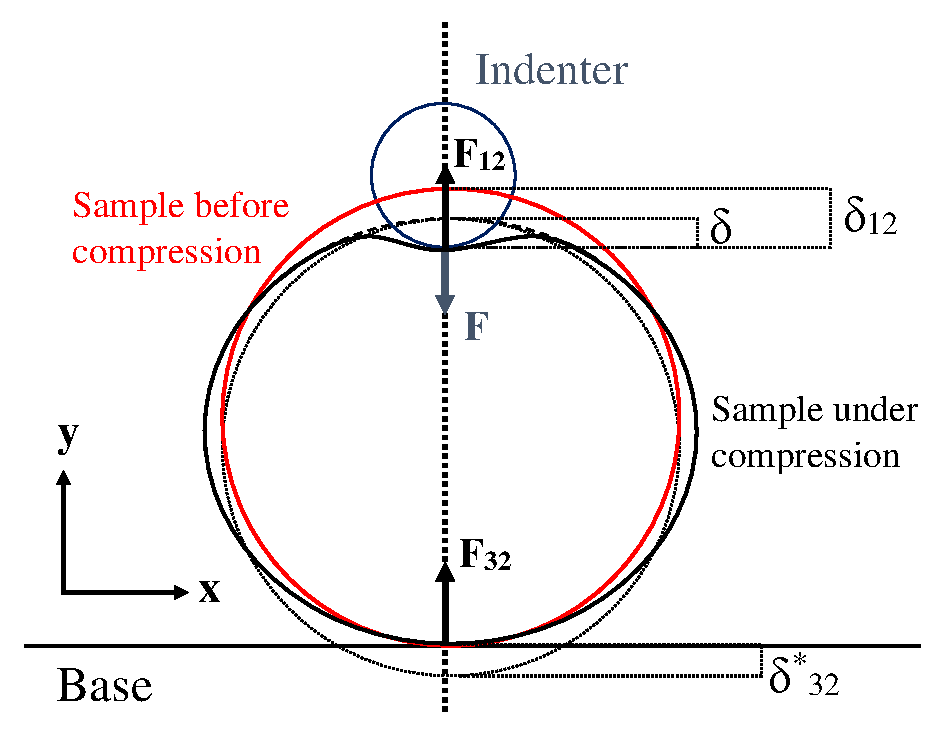
\includegraphics[width=1\linewidth]{Figures/Double Contact.pdf}
    \end{subfigure}
    \hfill
    \begin{subfigure}[t]{0.45\textwidth}
        \centering
        \caption{\label{fig: Sphere-Sphere_ABAQUS-Result}}
        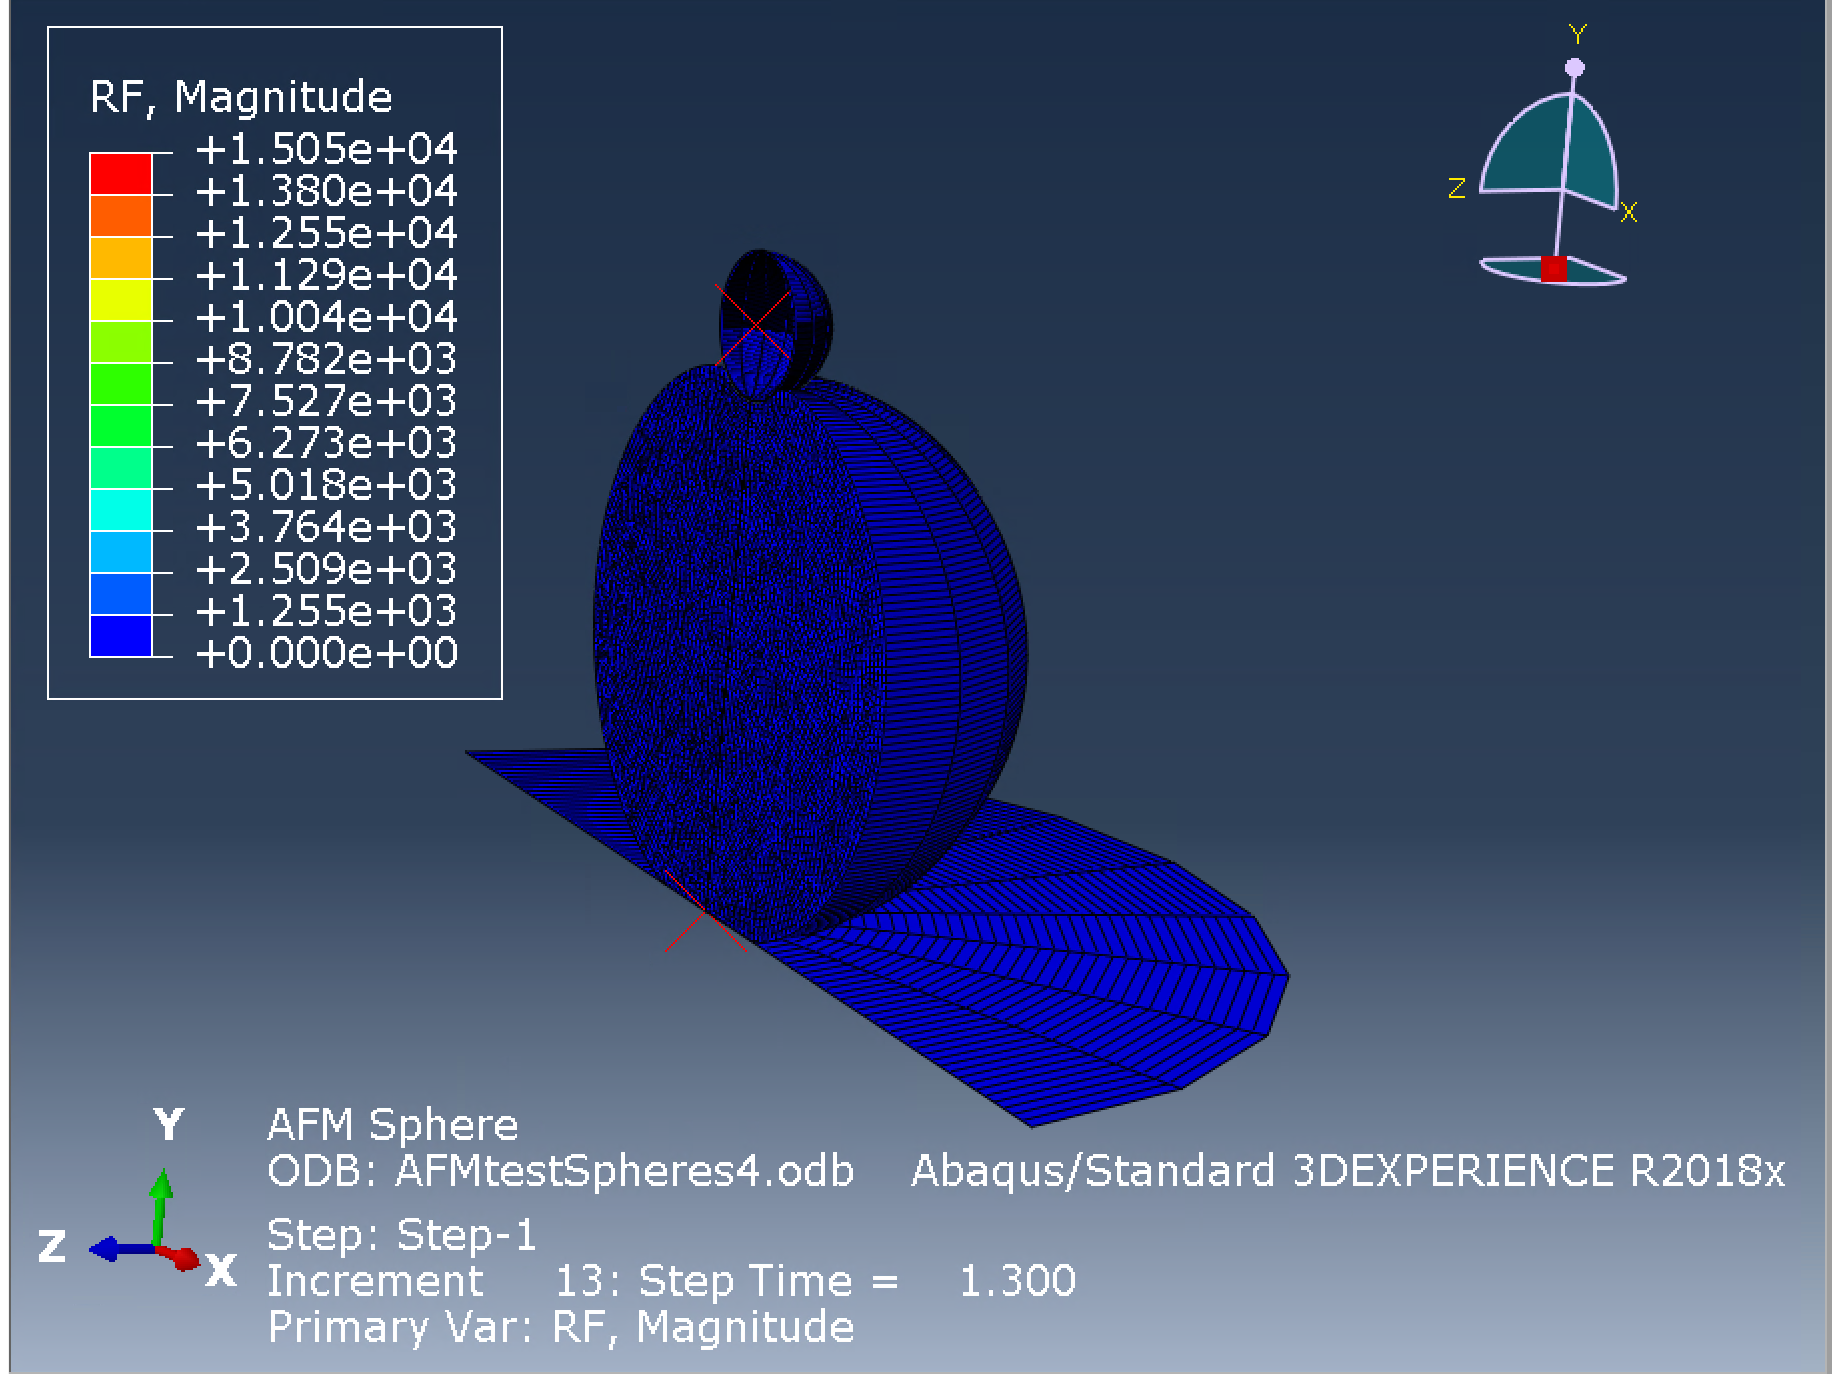
\includegraphics[width=1\linewidth]{Figures/Sphere-Sphere_Result.png}    
    \end{subfigure}

    \hfill

    \begin{subfigure}[t]{0.45\textwidth}
        \centering
        \caption{\label{fig: Sphere-Sphere-Force_Curve} }
        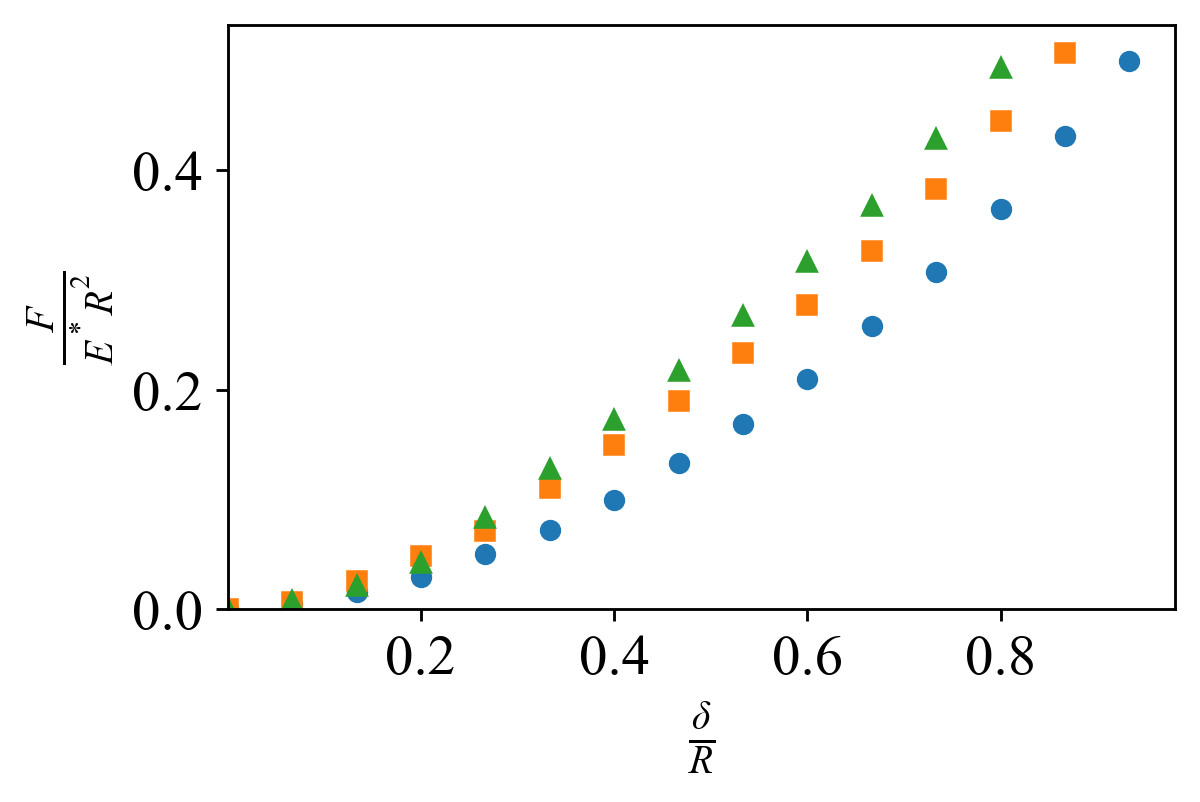
\includegraphics[width=1\linewidth]{Figures/Sphere-Sphere-Force_Curve-Indenter.png}
    \end{subfigure}
    \hfill
    \begin{subfigure}[t]{0.45\textwidth}
        \centering
        \caption{\label{fig: Sphere-Sphere-Force_Curve-Base} }
        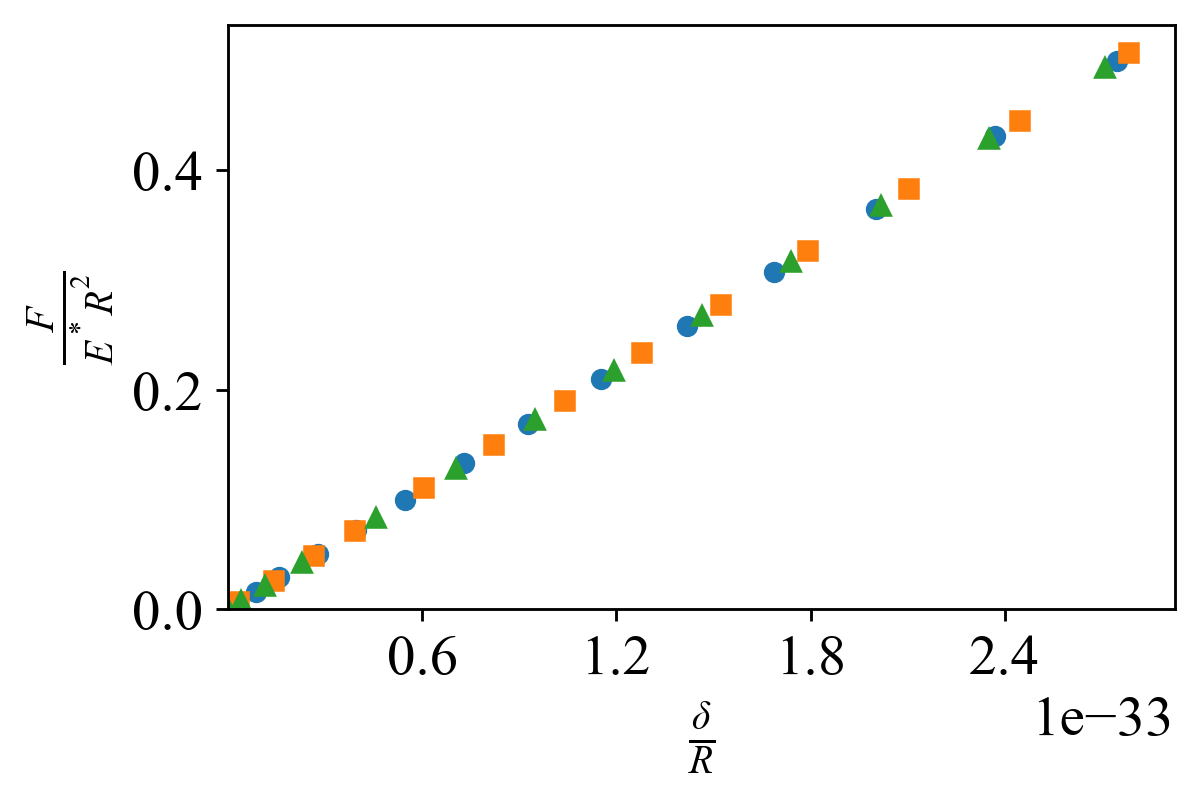
\includegraphics[width=1\linewidth]{Figures/Sphere-Sphere-Force_Curve-Base.png}
    \end{subfigure}

    \hfill
    
    \begin{subfigure}[t]{1\textwidth}
        
\includegraphics[width=1\linewidth]{Figures/Spheres-Force_Curve-Legend.png}
    \end{subfigure} 

    \caption{\label{fig: Sphere-Sphere-Result}(A) Illustration of double contact experienced by spherical sample. For indentation $\delta$, indenter displacement $\delta_{12}$, surface compression $\delta^*_{32}$, indentation force $F$, indenter reaction force $F_{12}$, and base reaction force $F_{32}$. (B) GUI visualisation for the sphere-sphere indentation where the asymmetric model is rotated 180 degrees around the central axis. (C) Force curve for spherical indentation $\delta/R$ into the elastic sphere of varying radius, r/R. (D) Force curve for compression of the surface into the base. Conical and capped indenter data is not shown, however, shows similar trends as before.}
    
\end{figure}

As shown in Figure \ref{fig: Sphere-Sphere-Youngs_Modulus}, the double contact models converged on the expected value for a spherical indenter. However, the error in the fit fluctuates as the surface radius increases. At small surface radii, excessive amounts of compression cause significant error and deviation from the theoretical models. The error decreases as the radius of the surface increases and compressive effects lessen; however, the error increases again at large surface radii as the geometry approximates an elastic half-space, and the double contact model is no longer valid. In contrast, errors in the Hertz and Dimitridias models decrease as the surface curvature decreases and the surface approximates an elastic half-space.

The Hertz model converged close to zero for the conical indenter shown in Figure \ref{fig: Cone-Sphere-Youngs_Modulus}. This indicates that the model diverges to large extents, which is expected as the Hertz model is for spherical indenters and an elastic half-space. On the other hand, the Sneddon model for the conical indenter converged to around 0.5. As discussed before, this is due to the compression of the sample, which reduced the reaction force at the tip. In contrast, applying a novel formulation of the Double Contact model for conical indenters (shown in Appendix \ref{Appendix: Sneddon Double}) produces a tight fit to the actual value across all surface radii.

\begin{figure}[H]
\centering

    \begin{subfigure}[t]{0.32\textwidth}
        \centering
        \caption{\label{fig: Sphere-Sphere-Setup}}
        \includegraphics[width=1\linewidth]{Figures/Sphere-Sphere-Setup.png}
    \end{subfigure}
    \hfill
    \begin{subfigure}[t]{0.32\textwidth}
         \centering
        \caption{\label{fig: Sphere-Sphere-Contact_Models} }
         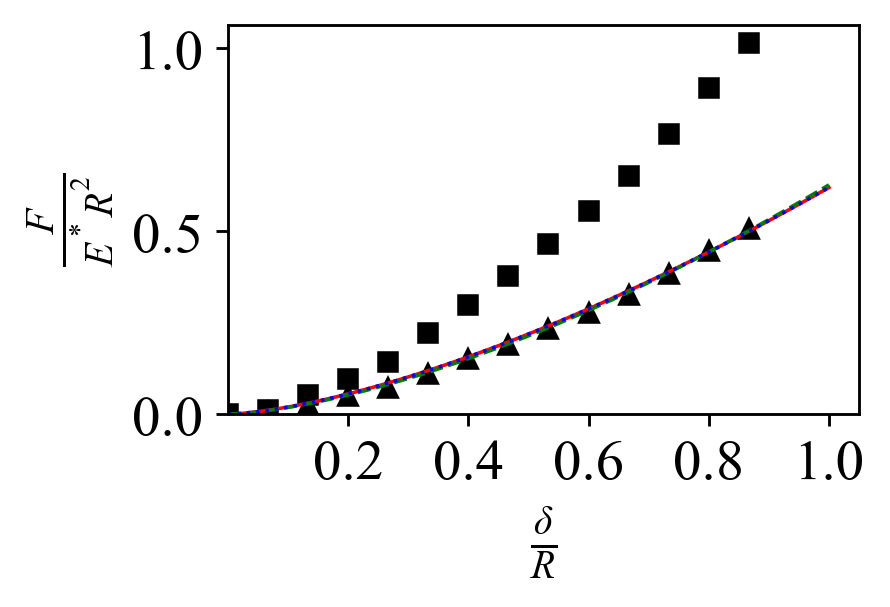
\includegraphics[width=1\linewidth]{Figures/Sphere-Sphere-Contact_Models.png}
    \end{subfigure}
    \hfill
    \begin{subfigure}[t]{0.32\textwidth}
        \centering
        \caption{\label{fig: Sphere-Sphere-Youngs_Modulus} }
        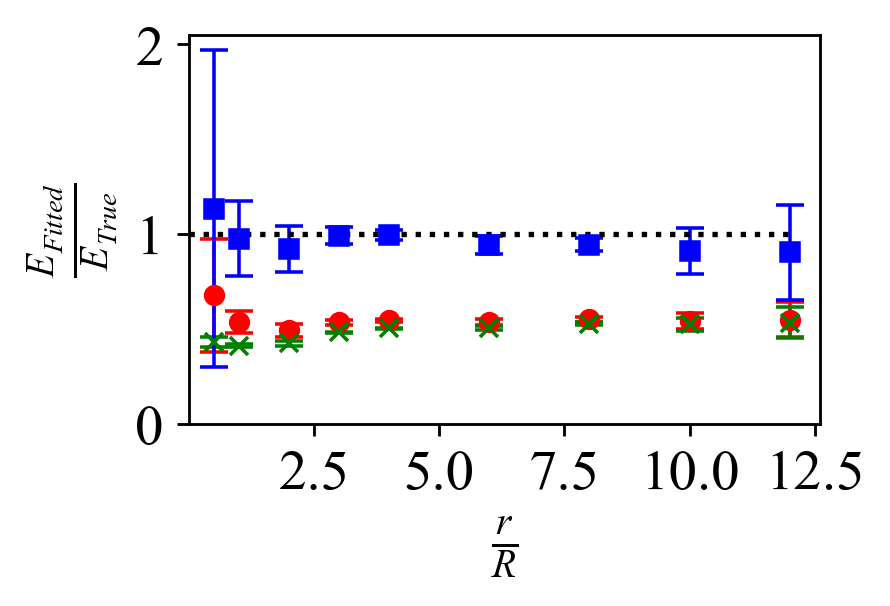
\includegraphics[width=1\linewidth]{Figures/Sphere-Sphere-Youngs_Modulus.png}
    \end{subfigure}
    
    \hfill
    \vspace{-0.4in}
    
    \begin{subfigure}[t]{0.32\textwidth}
        \centering
        \caption{\label{fig: Capped-Sphere-Setup}}
        \includegraphics[width=1\linewidth]{Figures/Capped-Sphere-Setup.png}
    \end{subfigure}    
    \hfill
    \begin{subfigure}[t]{0.32\textwidth}
        \centering
        \caption{\label{fig: Capped-Sphere-Contact_Models}   }
        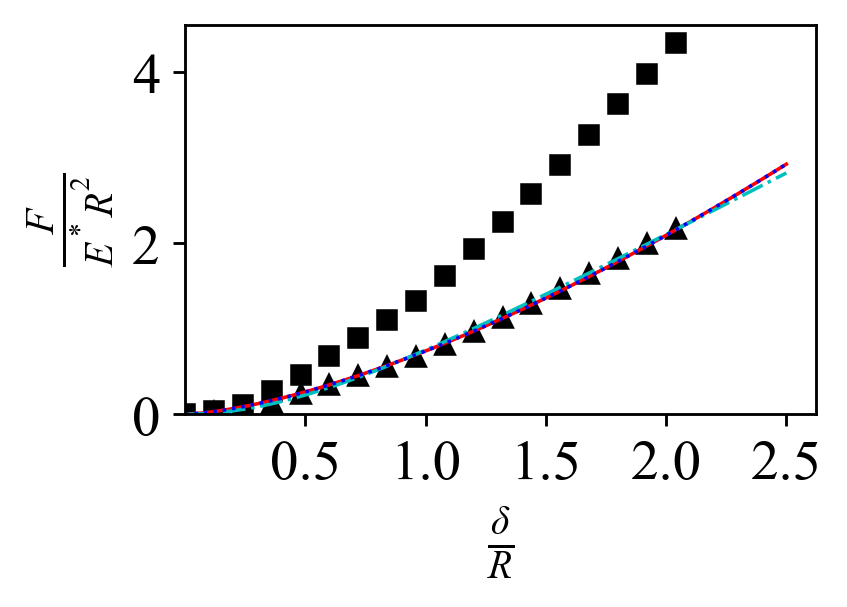
\includegraphics[width=1\linewidth]{Figures/Capped-Sphere-Contact_Models.png}
    \end{subfigure}
    \hfill
    \begin{subfigure}[t]{0.32\textwidth}
        \centering
        \caption{\label{fig: Capped-Sphere-Youngs_Modulus} }
        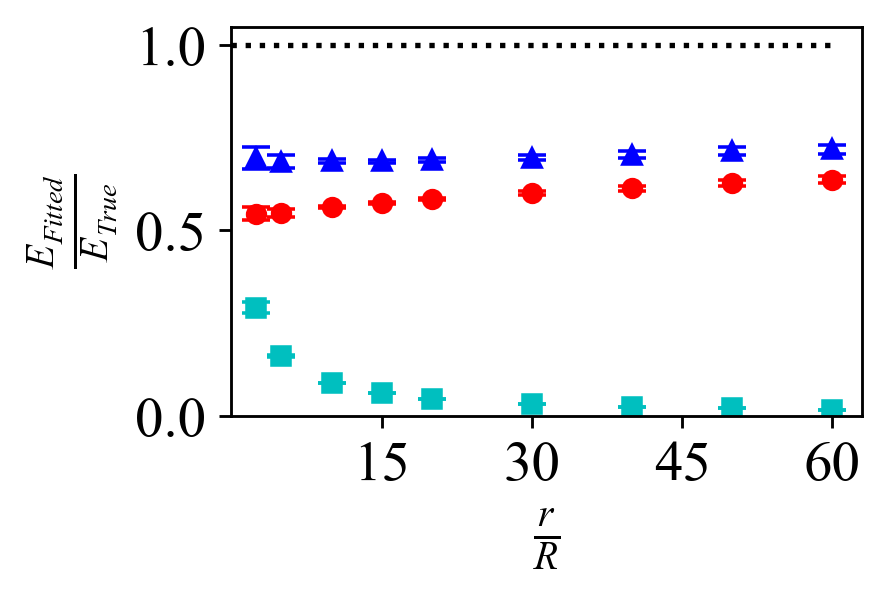
\includegraphics[width=1\linewidth]{Figures/Capped-Sphere-Youngs_Modulus.png}
    \end{subfigure}

    \hfill
    \vspace{-0.4in}
    
    \begin{subfigure}[t]{0.32\textwidth}
        \centering
        \caption{\label{fig: Cone-Sphere-Setup}}
        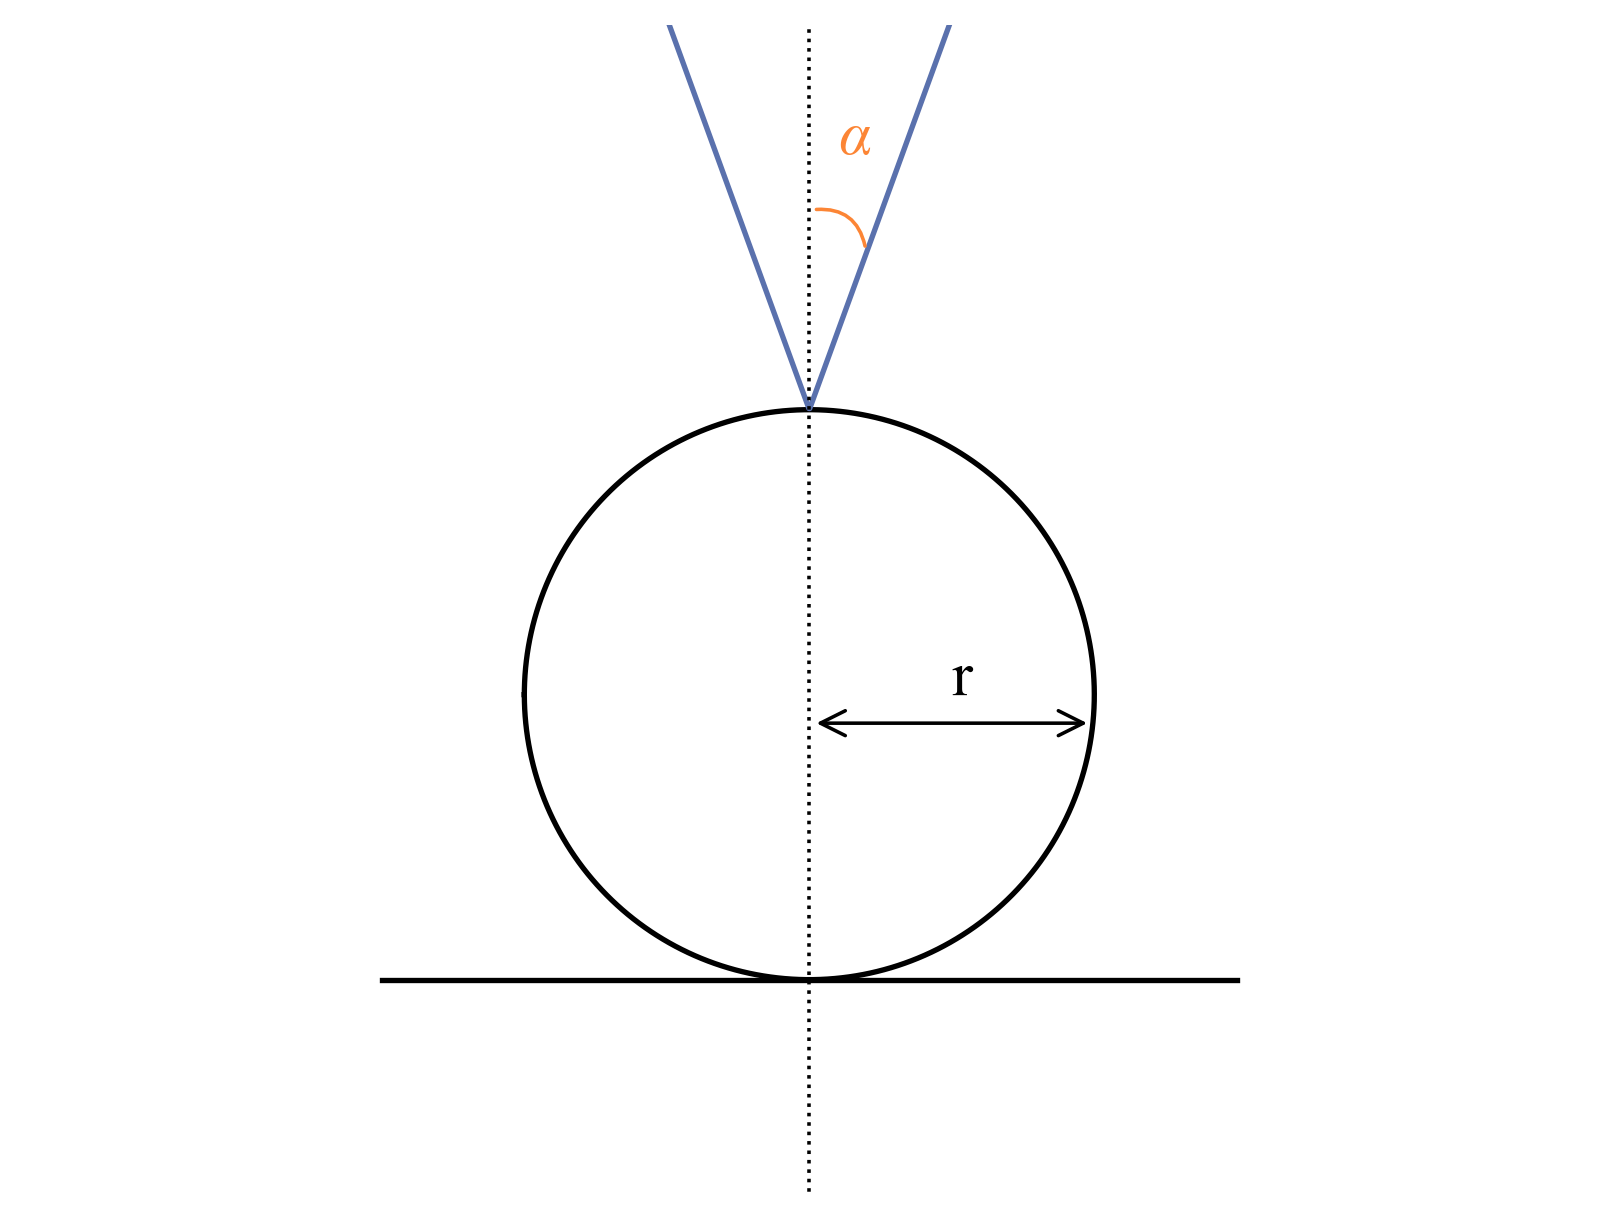
\includegraphics[width=1\linewidth]{Figures/Cone-Sphere-Setup.png}
    \end{subfigure}
    \hfill
    \begin{subfigure}[t]{0.32\textwidth}
        \centering
        \caption{\label{fig: Cone-Sphere-Contact_Models} }
        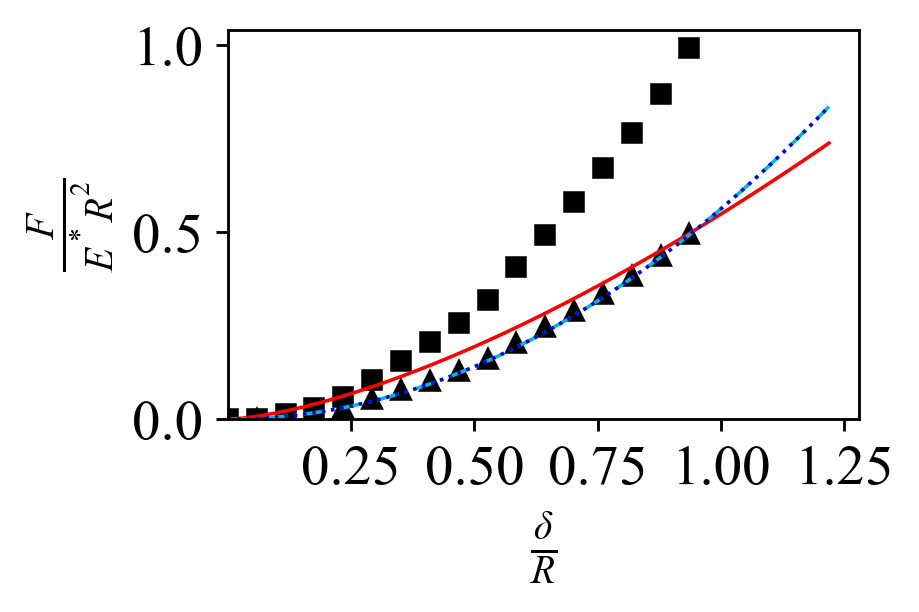
\includegraphics[width=1\linewidth]{Figures/Cone-Sphere-Contact_Models.png}
    \end{subfigure}
    \hfill  
    \begin{subfigure}[t]{0.32\textwidth}
        \centering
        \caption{\label{fig: Cone-Sphere-Youngs_Modulus} }
        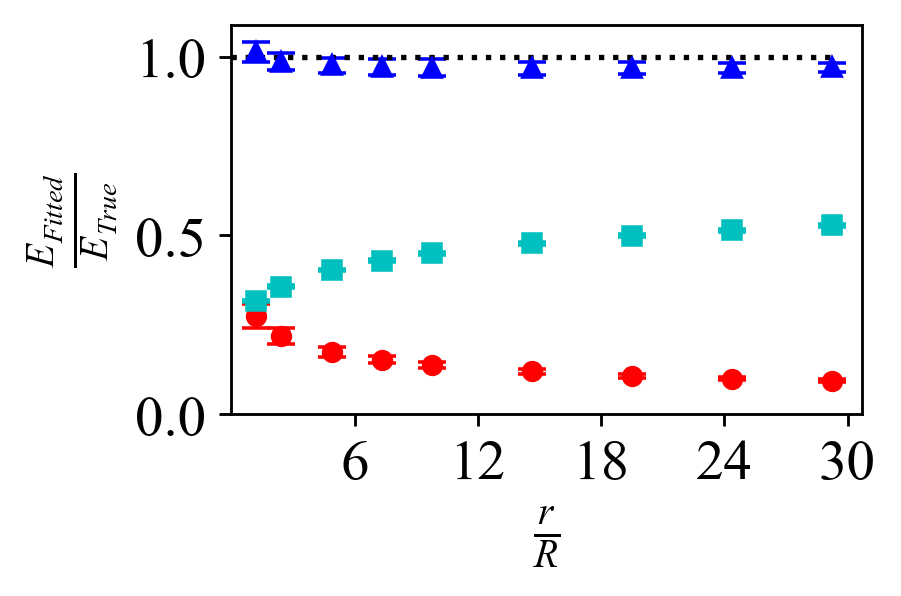
\includegraphics[width=1\linewidth]{Figures/Cone-Sphere-Youngs_Modulus.png}
    \end{subfigure}

    \hfill
    
    \begin{subfigure}[t]{1\textwidth}
        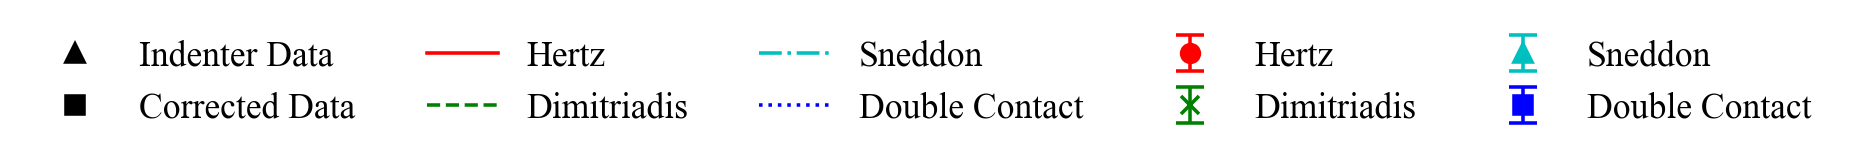
\includegraphics[width=1\linewidth]{Figures/Spheres-Legend.png}
    \end{subfigure}

    
    \caption{\label{fig: Sphere-Contact_Models}(A) Model assembly for spherical indentation of the elastic sphere. (B) Plot for spherical indentation force curves fitted using the Hertz, Dimitridias, and Double Contact models. (C) Youngs Modulus variation for spherical indentation into an elastic sphere. (D) Model assembly for spherically-capped conical indentation of an elastic sphere. (E) Plot for capped indentation force curves fitted using the Hertz, Sneddon, and Double Contact models. (F) Youngs Modulus variation for capped conical indentation into an elastic sphere. (G) Model assembly for conical indentation of an elastic sphere. (H) Plot for conical indentation force curves fitted using the Hertz, Sneddon, and Double Contact models. (I) Youngs Modulus variation for conical indentation into an elastic sphere. For conical indenter data normalisation, $R=\delta_{max}\tan(\alpha)$. Conical and capped indenters have the same dimensions as used in half-space simulations.}
    
\end{figure}
 
In comparison, for the capped indenter, the Double Contact model converged around 0.75. This offset is expected because the non-spherical portion of the indenter produces less curvature and deviation from the theoretical model. Similarly, the deviation produced by compression at the base leads to a similar convergence in the Hertz model. In comparison, the Sneddon model shows poor fit as it converges to 0. This indicates that the spherical indentation is dominant at these depths. Overall, these results further validated our ABAQUS modelling.

%%%%%%%%%%%%%%%%%%%%%%%%%%%%%%%%%%%%%%%%%%%%%%%%%%%%%%%%%%%%%%%%%%%%%%%%%%%%z